\documentclass{NSF}


  \usepackage[T1]{fontenc} 
    \usepackage{textcomp} 
   \usepackage{mathpazo} 
   \usepackage{framed}
   
%%%%%%%%%%%%%%%%%%%%%%%%%%%%%%%%%%%%%%%%%%%%%%%%%%%%%%%%%%%%%%%%%%%%%%%%%
%\pagestyle{plain}                                                      %%
%%%%%%%%%% EXACT 1in MARGINS %%%%%%%                                   %%
% %\setlength{\textwidth}{6.5in}     %%                                   %%
% \setlength{\oddsidemargin}{0in}   %% (It is recommended that you       %%
% \setlength{\evensidemargin}{0in}  %%  not change these parameters,     %%
% \setlength{\textheight}{8.5in}    %%  at the risk of having your       %%
% \setlength{\topmargin}{0in}       %%  proposal dismissed on the basis  %%
% \setlength{\headheight}{0in}      %%  of incorrect formatting!!!)      %%
% \setlength{\headsep}{0in}         %%                                   %%
% \setlength{\footskip}{.5in}    

\usepackage{epstopdf}
\epstopdfDeclareGraphicsRule{.gif}{png}{.png}{convert gif:#1 png:\OutputFile}
\AppendGraphicsExtensions{.gif}
\usepackage{rotating}
\usepackage{framed}
\usepackage{colortbl}
\usepackage{wrapfig}

\usepackage{pgfplots}
 
\newcommand{\IT}{{\bf {\sffamily TINKER}}}
\definecolor{maroon}{cmyk}{0,0.87,0.68,0.32}
\setlength{\parskip}{0.5mm}
\usepackage{indentfirst}
\setlength{\parindent}{0.75cm}


\newcommand{\quart}[4]{\begin{picture}(80,4)%1
    {\color{black}\put(#3,2){\circle*{4}}\put(#1,2){\line(1,0){#2}}}\end{picture}}

\usepackage{longtable}
\usepackage[most]{tcolorbox}
\usepackage{caption}
\usepackage{multirow}
\usepackage{comment}
\usepackage{pifont}
\usepackage{array}
\usepackage{enumitem}

\newenvironment{myitemize}
{ \begin{itemize}
    \setlength{\itemsep}{0pt}
    \setlength{\parskip}{0pt}
    \setlength{\parsep}{0pt}     }
{ \end{itemize}                  } 


\newenvironment{mysmallize}
{ \begin{itemize}[leftmargin=*,topsep=0pt]
    \setlength{\itemsep}{0pt}
    \setlength{\parskip}{0pt}
    \setlength{\parsep}{0pt}     }
{ \end{itemize}                  } 


\newenvironment{mynumns}
{ \begin{enumerate}
    \setlength{\itemsep}{0pt}
    \setlength{\parskip}{0pt}
    \setlength{\parsep}{0pt}     }
{ \end{enumerate}   }
 
 \definecolor{ao(english)}{rgb}{0.0, 0.5, 0.0}
    

\newcommand{\be}{\begin{mynumns}}
\newcommand{\ee}{\end{mynumns}}

\newcommand{\bi}{\begin{myitemize}}
\newcommand{\ei}{\end{myitemize}}


\newcommand{\bii}{\begin{mysmallize}}
\newcommand{\eii}{\end{mysmallize}}

\newcommand{\tion}[1]{\S\ref{tion:#1}}

\newcommand{\tbl}[1]{Table~\ref{tbl:#1}}
\newcommand{\fig}[1]{Figure~\ref{fig:#1}}

\newcommand{\eq}[1]{Equation~\ref{eq:#1}}

\usepackage[T1]{fontenc} 
\usepackage{textcomp} 
\usepackage{mathpazo} 
   

\definecolor{Gray}{gray}{0.9}

\hyphenation{}

\newcommand{\jnote}[1]{{\color{blue}[JEFF: #1]}}

\newcommand{\IT}{{\bf {\sffamily TINKER}}}
\newtheorem{criteria}{Evaluation Criteria}

\usepackage[tikz]{bclogo}

\usepackage{tikz}
\def\checkmark{\tikz\fill[scale=0.3](0,.35) -- (.25,0) -- (1,.7) -- (.25,.15) -- cycle;} 
\def\firstcircle{(90:1.75cm) circle (2.5cm)}
\def\secondcircle{(210:1.75cm) circle (2.5cm)}
\def\thirdcircle{(330:1.75cm) circle (2.5cm)}

\newenvironment{eval}[1]%
{\noindent\begin{minipage}[c]{\linewidth}%
\begin{bclogo}[couleur=gray!25,%
                arrondi=0.1, 
                barre=zigzag,%
                logo=\bcattention,%
                ombre=true]{~#1}\begin{criteria}}%
{\end{criteria}\end{bclogo}\end{minipage}\vspace{2mm}}

\newcommand{\TITLE}{FAI:  Fairness is a Choice But Not
Choosing is Unfair (The TINKER Project)}

 \usepackage[labelfont=bf,font=bf]{caption}
 \captionsetup{font+=sf}
               
               
   
\begin{document}
\ProjectTitle{\TITLE}
\ProjectAuthor{Tim Menzies, NC State}

%\renewcommand{\attn}
 
\begin{nsfsummary}
\begin{center}
{\bf \TITLE}\\\vspace{1mm}
 Tim Menzies,  IEEE Fellow, NC State
 \end{center}
   Recent results warn that the software within many data mining packages exhibits "group discrimination"; i.e. their decisions are inappropriately affected by protected attributes (e.g., race, gender, age, etc.). 
  We assert that it is the ethical duty of software designers to strive to reduce  discrimination. This research discusses how that might be done. %There have been a research on fairness and algorithmic transparency in machine learning. Different groups apply different fairness operators to enhance their data miners. But the experience to date is that some of these operators lead to unacceptable loss in learner performance. 
  
  We observe that, during learning, {\bf if fairness is not known to be a goal}, then {\bf the learner will not generate fair models}. To fix this problem we propose moving the fairness goal into the model generation process. Specifically, we will explore if 
  {\bf  hyper-parameter optimization} can automatically find tunings for learners such that they generate fair modes without losing predictive performance. Our preliminary results are promising. We have shown that  hyper-parameter optimization can (a) preserve the predictive power of a model learned from a data miner while also (b) generates fairer results. 
  
  That said, our
  hyperparameter optimization methods are resource expensive. Hence, to support    widespread fariness via hyper-parameter optimization , we need to find linear (or sub-linear) time optimizers. 
  For this research we will explore how   {\em not} to tune from scratch.
  Rather, we will bootstrap the  tuning
  process by  {\em transferring}, then {\IT}ing with  old tunings.
  
  
  %(where fairness is measured by the standard metrics suite supported by the AIF360 fairness suite https://github.com/IBM/AIF360). To the best of our knowledge, ours is the first application of hyper-parameter optimization as a tool for software engineers to generate fairer software. 
 



\vspace{2mm}
 \noindent
\underline{{\bf INTELLECTUAL MERIT:}} 
Our work speaks to a core issue in AI: how to trust automatically generated models.
``Trust'' means   different things to different people but, at the very least, we should
demand that  our AI models are not needlessly discriminating against specific social groups.

As to other merits,  too much prior work has focused on  model  performance 
while disregarding any inherent bias the model is introducing in decision making. The methods in this proposal could be used to better understand the discrimination introduced in decision making by models and ways to remove this without suffering from performance bottleneck.

Further, {\IT} method for speeding up hyperparameter optimization (via transfer) should
be broadly applicable to many domains such as AI+fairness as well as any other domain that uses
machine learners. To say the least, there are many such domains
 
 
\vspace{2mm}
\noindent
\underline{{\bf BROADER IMPACTS:}}
We focus on an issue of tremendous socio economical importance - many high-stake applications such as finance, hiring, admissions, criminal justice use algorithmic decision-making frequently. In some cases, machine learning models make better decisions than human can do. But there are many scenarios where machine learning software has been found to be biased and generating arguably unfair decisions. For industrial and academic sectors, this work proposes a fairness testing and optimizing for every machine learning model to generate fairer results, thus removing the ``discrimination problem''.

PI Menzies will continue his established tradition of graduating research students for historically under-represented groups. This work will inform the curriculum of  the various NC State  NSF-funded REUs (research experience for undergraduates).
In that program, places are reserved for students from traditionally under-represented areas; e.g. economically challenged regions of the state of North Carolina) and/or students from universities lacking advanced research facilities. While some of the concepts of this grant would be too advanced for that group, some of the simpler concepts and case studies would be suitable for lectures.

\vspace{2mm}
\noindent \underline{{\bf KEYWORDS:}} fairness, empirical software engineering, software analytics
\end{nsfsummary}


\begin{nsfdescription}
\thispagestyle{plain}
 \begin{center}
{\bf \TITLE}\\
{Tim Menzies,  IEEE Fellow,  NC State}
 \end{center}


 

 \section{Introduction}\label{tion:intro}
We assert that it is the ethical duty of anyone building
software   to strive to reduce any discrimination inherent in that software. This research discusses how that might be done.



\begin{wraptable}{r}{3.2in}
\begin{tabular}{|p{3in}|}\hline
\rowcolor{gray!20}\small
\begin{itemize}[leftmargin=*]
\item
Google's sentiment analyzer model  which determines positive or negative sentiment, gives negative score to   sentences like \textit{`I am a Jew', and `I am homosexual'}\cite{Google_Sentiment}. 
\item
Facial recognition software which predicts characteristics such as gender, age from images has been
found to have a much higher error rate for dark-skinned women compared to light-skinned men \cite{Gender_Bias}. 
\item
A popular photo tagging app   assigns animal category labels to dark skinned people \cite{Google_Photo}. 
\item 
Some recidivism assessment models used by the criminal justice system         are more likely to falsely label black defendants as future criminals (at  twice the rate as white defendants) \cite{Machine_Bias}. 
\item
Amazon.com stopped using automated  recruiting tools after finding anti-women bias\cite{Amazon_Bias}. 
% \item
% Cathy O'Neil provided even more examples of unfair decisions made by software in her book ``Weapons of Math Destruction''\cite{O'Neil:2016:WMD:3002861}. She argued that machine learning software generates models that are full of bias. Hence, this is one of the reasons their application results in unfair decisions.
\end{itemize}\\\hline
\end{tabular} 
\caption{Recent high-profile examples of software with inherent discriminatory properties.}
\label{tbl:eg}
\end{wraptable}
Software is increasingly being used to make decisions that affect people's lives. 
 Machine learning models are used to support decision making in high-stakes applications such as mortgage lending, hiring, and prison sentencing. 
Many high-stake applications such as finance, hiring, admissions, criminal justice use algorithmic decision-making frequently~\cite{ladd1998evidence,burrell2016machine,corbett2018measure,galindo2000credit,yan2013system,chalfin2016productivity,ajit2016prediction,berk2015machine,berk2016forecasting,ozkan2017predicting}. 
Unfortuneately, some of that software is known to  exhibit ``group discrimination''; i.e. their decisions are inappropriately affected by protected attributes; e.g., race, gender, age, etc.  (see \tbl{eg}).

There has been much recent work on validating the fairness of machine-learning models (by recognizing when such software discrimination exists). For example, in the arena of software engineering, 
Tramer et al. proposes different ways to measure discrimination \cite{Tramer_2017}.
  %Angell et al. \cite{Angell:2018:TAT:3236024.3264590}  note that     ``fairness'' is analogous to other measures of software quality. 
  Galhotra et al discuss how to efficiently generate test cases to test for discrimination\cite{Galhotra_2017}.  Udeshi et al. \cite{Udeshi_2018} find they can
  generating discriminatory  inputs for machine learning software.  Albarghouthi et al. \cite{Albarghouthi:2019:FP:3287560.3287588} explore if fairness can be wired into annotations within a program.
 
 
 While all this work is certainly useful, it is incomplete. After unfairness
 is {\em detected}, the next step must be {\em mitigation}; i.e. the reduction of the
 detected unfariness.
 Hence, we ask,
 what tools can ethical software developers take to reduce discrimination in the software they produce?

Our tool for increasing fairness is {\em hyperparameter optimization}. 
Such optimizers explore the control parameters of a learner. In this way, they can generate and validate
many models per minute (depending on the size of the data and
the training time of the learner). Such optimizers
are executed with particular goals in mind (e.g. reduce false alarms and improve precision). 
Based on our experience with such optimizers, we say that  data set can be fitted to multiple models (just by altering the control parameters of the machine learners).
Also, as shown by the experiments presented later in this proposal, it is possible for such optimizers
to find fairer models\footnote{Where ``fair'' is determined by measures like those
presented in \tion{XXX}.}.
However, only a small fraction of the models generated in this way maintain fairness.
That is, 
{\bf if fairness is not known to be a goal}, then {\bf the optimizer is unlikely to generate fair models}.
Hence we say:
\bi
\item {\em Fairness is a choice}. Data scientists
can decide whether or not to use   hyperparamter optimziation
to find fair models.
\item {\em But not choosing is unfair.}
If data scientists do not optimize for fairness,
and select models using (say) the default control
parameters of the learner, then it is most
likely they will end up with an unfair model
(since only a small fraction of the models maintain
fairness).
\ei
XXX

\section{Case Study: Mitigating Unfairness in ``Model Stores''}
Given recent advances in software development,
it is now an open and 
urgent problem to detect and mitigate
  group discrimination in machine learning models.
  This describes those advances. In summary,
  
  \begin{figure}
 \centering 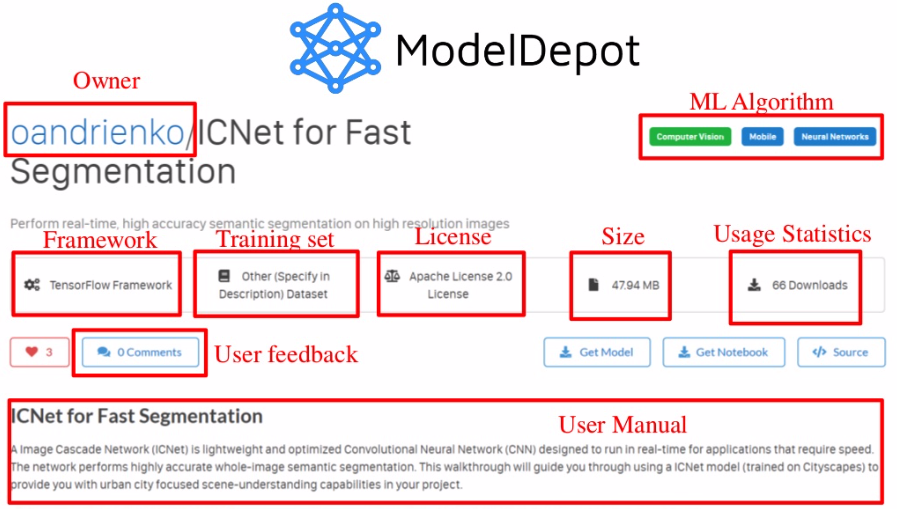
\includegraphics[width=5in]{fig/store.png}
 
  \caption{One of the machine learning models
  available for rent from the ModelDepot model store.
  Note that hundreds of such models
  are currently available (see \tbl{stats})
  and that number is rapidly growing.}\label{fig:one}
  \end{figure}
  
  It is now trivial to package and distribute even
  the most complex machine learning process
  as containers executing in the cloud.
   Specifically,
   it is now a mere matter of hours to take a Github repo with some example shell  scripts, and turn that code into a cloud-based application\footnote{E.g. see opendatahub.io's machine-learning-as-a-service platform based on Kupernetes that can rapidly transfer Juypter notebooks (developed locally)  to cloud-based
  execution environments.}.
  Hundreds of
  such containers are now available for rent, in
  ``model stores'' at  AWS marketplace XX;
  Wolfram neural net repository ZZ;  and  the  ModelDepot YY
(see \tbl{stats}).  Users can
rent these models, as well as the cloud-CPU required
to execute them. In this arrangement, users upload their data to the cloud-based model. Then, later on,
they download the generated model. 

These tools have simplified the generation and distribution of machine learning models.
However, regrettably, they have also made it much simpler to 
unwittingly  distribute  software that exhibits
``group discrimination''.  The model store sites caution
users to beware biases in their model generation methods, or the generated model. However, they offer no tools for detection   such bias, or mitigating such bias (if it exists). This is despite the fact
that many of these models contain attributes that we might want to detect.
For example, to support this proposal, we sampled 32 models at random from
the AWS model store. We found several eight models that  that could could inappropriately target protected social groups (e.g. age, gender or race). A sample of those models are shown in \tbl{msample}
\begin{table}
\small
\begin{tabular}{|p{0.8in}|p{5.4in}|}\hline
\rowcolor{gray!20}
 {\em hyScore} & {\em hyScore} is an NLP tool which, amongst other things, performs  sentiment analysis of content. hyScore accepts arbitrary free form text which, potentially, could reference   social groups we might want to protect.
 \\ 
 {\em  Credit Default Predictor} &{\em Credit Default Predictor} uses   23 attributes include gender, education. age, and previous history of payments to generate an   predictor of the chances a customer will default on a loan
 \\
\rowcolor{gray!20}
{\em Hospital Readminission} &
The decision whether or not to discharge a patient can be a life or
death decision since, if the wrong patient's are discharged, they
will not have access to   intra-hospital services if they have an acute medical event. The {\em Hospital Readminission} model predicts the probably that a patient will not be readmitted after discharge. This model's inputs include financial class, sex and age. Depending on the protected attributes a hospital may decide not to release the patient as the model shows high probability of readmission, while another patient with same other attributes but different protected attribute values can be released.
\\
\hline
\end{tabular}
\caption{A sample of models that from the AWS model store
that might  could inappropriately target protected social groups (e.g. age, gender or race). Note that this list is based on a quick survey
of 32 of the 300+ models currently available on-line.
Based on this survey, we conclude that many of Model Store
applications could produce unfair models.}\label{tbl:msample}
\end{table}


Paradoxically,   Model Stores are both the worst and best thing to happen to model fairness. On the one hand, they have the potentially to make the mode; fairness problem much worse as more models are used uncritically
by consumers who are unaware of the biases of those models.
But on the other hand, Model Stores have the potentially to dramatically simplify the problem of generating fair models. 

To understand this point, consider the following three points.
Fristly, as shown later in this proposal, if a hyperparameter optimizers
is aware of fairness goals, then those optimizers can generate models
that good predictors without also being unfair to social groups we might wish to predict.

Secondly,  hyperparameter optimization slows down the process of model generation. Naive optimizers may require thousands to millions of executions of a learner\footnote{e.g. grid search}. Smarter optimization strategies require fewer executions\footnpte{e.g Bayes parameter optimization} but even here, tens to hundreds of executions might be required. For large data sets or slow learners, this can be unacceptable especially when the user of the machine learner is paying for the cloud CPU time required to learn the model. 

Thirdly


While this a
  
it is now trivial to deploy even
the most complex machine learning method. 

This section
describes those advances as well as what that means
for packaging and distributing machine learning models.
In summary 
It 


  Various crowd computing vendors are now running ``model store'' where customers
  rent cloud CPU time to run their data through cloud-based machine learning apps. Xie et al.~\cite{xiu2019exploratory} report that  
  now offer 339 models (see \tbl{stats}). 
  
Due to recent advances in software development,
we can reasonably expect that the number of such models will increase very    increasing. At the SEMLA'19 meeting~\cite{semla19}
the software distribution company Redhat described how they are
teaming with many organizations to streamline ``containerization'' services. ``Containers'' are ways to wrap up and disseminate to the cloud sets of software services. While the services themselves may be complex to build, for the user of the container, it is just a matter of loading and running the container on their favorite cloud service provider. 

hat are 
\begin{wraptable}{r}{4in} 
%\begin{table}[]
\begin{tabular}{p{1.5in}p{0.5in}p{0.5in}p{0.5in}} \hline
\rowcolor{blue!10}Group & AWS & Model Depot & Wolfarm \\ \hline
Image & 61 & 24 & 59 \\ \hline
\rowcolor{blue!10}Video & 13 & 2 & 0 \\ \hline
Natural language texts & 35 & 5 & 18 \\ \hline
\rowcolor{blue!10}Audio & 12 & 1 & 2 \\ \hline
Strctured & 107 & 0 & 0 \\ \hline
\rowcolor{blue!10}Total & 228 & 3 & 79 \\ \hline
\end{tabular}
%\end{table}
  \caption{As of June 2019, there are 339 models
  for hire at on-line model stores.
   Note
  that the number of models at these sites is growing rapidly.}
  \label{tbl:stats}
  \end{wraptable}
Issues of machine learning model 
a small fraction of   possible models say that {\e fairness is a choice}
e observe t set and the shat, during learning of the data,  To fix this problem we propose moving the fairness goal into the model generation process. Specifically, we will explore if 
  {\bf  hyper-parameter optimization} can automatically find tunings for learners such that they generate fair modes without losing predictive performance. Our preliminary results are promising. We have shown that  hyper-parameter optimization can (a) preserve the predictive power of a model learned from a data miner while also (b) generates fairer results. 
  
  That said, our
  hyperparameter optimization methods are resource expensive. Hence, to support    widespread fariness via hyper-parameter optimization , we need to find linear (or sub-linear) time optimizers. 
  For this research we will explore how   {\em not} to tune from scratch.
  Rather, we will bootstrap the  tuning
  process by  {\em transferring}, then {\IT}ing with  old tunings.
  
This paper shows that making fairness as a goal during hyperparamter optimization can (a) preserve the predictive power of a model learned from a data miner while also (b) generates fairer results. To the best of our knowledge, this is the first application of hyperparameter optimization as a tool for software engineers to generate fairer software.


 \section{Background}\label{tion:back}

Machine learning software, by its nature, is always a form of statistical discrimination. 
Those discrimination becomes objectionable when it places certain privileged groups at  a systematic advantage and certain unprivileged groups at a systematic disadvantage. In certain situations, such as employment (hiring and firing), discrimination is not only objectionable, but illegal.

Much resaerch In our own domain Issues of \textit{fairness} have been explored in many  recent papers in the SE research literature.
In summary, that work concludes that fairness is an important issue:
\bi
\item Angell et al. \cite{Angell:2018:TAT:3236024.3264590}  note that     ``fairness'' is analogous to other measures of software quality. \item Galhotra et al discussed how to efficiently generate test cases to test for discrimination\cite{Galhotra_2017}. \item Udeshi et al. \cite{Udeshi_2018} worked on generating discriminatory  inputs for machine learning software. \itemAlbarghouthi et al. \cite{Albarghouthi:2019:FP:3287560.3287588} explored if fairness can be wired into annotations within a program.
\item Tramer et al. proposed different ways to measure discrimination \cite{Tramer_2017}.
\ei
All the above SE research detects unfairness. Our work takes a step further and asks how to mitigate
unfairness. We propose that every machine learning model must go through fairness testing phase before it is applied. If bias is found, then the model needs to be optimized. Hence, we have converted ``discrimination problem'' into an optimization problem. We think that if \textit{fairness} becomes a goal while learning, then the  models created in that way will generate fairer results. In this study, we investigated whether model parameter tuning can help us to make the model fair or not. 
 
 In machine learning, many  {\em hyperparameters} control   inductive process ; e.g. the   `splitter' of CART~\cite{breiman2017classification}.  They are very important because they directly control the behaviors of the training algorithm and impact the performance of the model. Therefore, the selection of appropriate parameters plays a critical role in the performance of machine learning models. Our study applies \textit{hyperparameter optimization} to make a model fair without losing predictive power. So, it becomes \textit{multiobjective optimization} problem as we are dealing with more than one objective. 
 

 
With algorithmic decision making becoming the norm, the issue of algorithmic fairness has been identified as a key problem of interdisciplinary dimensions \cite{IBM} . Machine learning models are used to support decision making in high-stakes applications such as mortgage lending, hiring, and prison sentencing~\cite{ladd1998evidence,burrell2016machine,corbett2018measure,galindo2000credit,yan2013system,chalfin2016productivity,ajit2016prediction,berk2015machine,berk2016forecasting,ozkan2017predicting}. In recent years, researchers have found unfairness in ML models \cite{IBM}. It is high time to put a sincere effort to achieve fair decision making using ML models.

Current fairness research focuses on mainly two directions - detecting or measuring  the unfairness and mitigating the unfairness. Galhotra et al. proposed an approach to generate efficient test suites to measure software discrimination \cite{Galhotra_2017}. When it comes to mitigate unfairness in ML models, AI researchers are still confused as they need to deal with questions such as ``Should the data be debiased?'', ``Should new classifiers will be created that learn unbiased models?'', or ``Is it better to correct predictions from the model?''. 

 \begin{wrapfigure}{r}{4.8in} 
%\begin{table}[!b]
\caption{Sample of Previous Studies}
\small
 \begin{center}
\begin{tabular}{p{0.6in}|p{3.9in}}
    
   \rowcolor{blue!10} Datasets & Adult Census Income, German Credit, COMPAS\\
    \hline
    Metrics&Disparate impact\\
    &Statistical parity difference\\
    &Average odds difference\\
    &Equal opportunity difference\\
    \hline
    \rowcolor{blue!10}Pre-  & Re-weighing (Kamiran et al., 2012) \cite{Kamiran2012}\\
    \rowcolor{blue!10} processing& Optimized pre-processing (Calmon et al., 2017) \cite{NIPS2017_6988} \\
   \rowcolor{blue!10}  & Algorithms Learning fair representations (Zemel et al., 2013) \cite{pmlr-v28-zemel13}\\
    \rowcolor{blue!10} & Disparate impact remover (Feldman et al., 2015) \cite{Feldman:2015:CRD:2783258.2783311}\\
    \hline
   In-     & Adversarial debiasing (Zhang et al., 2018) \cite{Zhang:2018:MUB:3278721.3278779}\\
    processing& Algorithms Prejudice remover (Kamishima et al., 2012) \cite{Kamishima}\\
    \hline
   \rowcolor{blue!10}  Post-   & Equalized odds post-processing (Hardt et al., 2016) \cite{Hardt}\\
    \rowcolor{blue!10}processing & Algorithms Calibrated eq. odds postprocessing (Pleiss et al., 2017) \cite{NIPS2017_7151}\\
   \rowcolor{blue!10}  & Reject option classification (Kamiran et al., 2012) \cite{Kamiran:2018:ERO:3165328.3165686}\\
   
\end{tabular}
\end{center} 
\label{tbl:multicol}
%\end{table}
\end{wrapfigure}
 
 \tbl{multicol} shows a  quick summary of research into fairness. That table shows a sample of  the datasets, metrics, classifiers, and bias mitigation algorithms used and developed so far. In the literature, it is claimed that
adversarial debiasing works best\cite{Zhang:2018:MUB:3278721.3278779} (but as shown in Figure~1, discussed below, adversarial debiasing has certain drawbacks). The idea of adversarial debiasing is to include a variable for the group of discrimination and simultaneously learning a predictor and an adversary. The input to the network X, produces a prediction Y, while the adversary tries to model a protected variable Z. The objective is to maximize the predictor's ability to predict Y while minimizing the adversary's ability to predict Z. 

Our experience is that most of the fairness algorithms, including
adversarial debiasing   achieve fairness by damaging
predictive performance.  Fig.~1 shows that various fairness algorithms damage model accuracy to achieve fairness ( tested on  Adult Census Income with protected attribute - "Sex")~\cite{IBM}.
Therefore, it is an open and urgent research challenge to gain fairness without damaging the performance of the decision-making algorithm or ML model. 

Our preferred method for avoding 
% Sometimes, it is appropriate to call our  certain social groups. For example,
% we should expect our machine learning algorithms to warn that older people need extra monitoring
% for cardiac issues. That said, sometimes, such reports are trite summary of simplisttic correlations
% and not comments on deep issues with the data. 
In our experience, one data set can be fitted
to many models (just by changing the control parameters of the machine learner). Suppose:
\bi
\item
There are
$N$ models with equivalent predictive power;
\item
And a few  $M<N$ of those models do not make use of information
such as race, age, or gender. 
\item
In terms of the fairness evaluation measures defined below,
that means that now there are $M$ ``fair'' models and $N-M$ ``unfair'' models. 
\ei
Common practice is not generate multiple models for one data set. In our literature
reviews on this matter, we find that very few researchers recommend
the generating and exploring multiple
models. For example, in our review of  hyperparameter model optimization  we found that in of 200+ highly cited papers in the last decade,
only 20\% of them using hyperparameter optimation (i.e. the automatic exploration
of many models of control
parameters of a learner),

In that case, we say that ``fairness is a choice'' since a data scientist can choose
to deploy fair or unfair models. But since $N<N$ then that means if a data scientist
chooise also that since $M<N$ then we sautat
``not chooisin
With that 


At that point, the data scientist has a {\em choice} of using
models that call out certain social groups and those that do not. 


% Much recent empirical SE research has focused on this data, and how
% to leverage this kind of Github data to build software quality models~~\cite{commitguru, Kim08changes,catolino17_jitmobile,nayrolles18_clever,mockus00changeskeys,kamei12_jit,hindle08_largecommits}.

%  To simplify the creation and maintenance of computational science software, we   propose  the  {\IT}\footnote{ Short for 
% ``empirical \underline{SE} \underline{n}ow \underline{TRY}-ed on  computational science code''.} empirical software engineering workbench.
% {\IT} contains a set of automatic agents that read code and comments and test
% results from on-line repositories of computational science code.  {\IT} will advise:
% \bi
% \item[(a)] Where defects are hiding the code;
% \item[(b)] How to prioritize test cases (so tests  likely to fail are executed sooner); 
% \item[(c)] The appropriate number of programmers required
% for each project; 
% \item[(d)] Now to avoid spurious error messages (e.g. from static code analysis tools);
% \item[(e)] Other issues, if time permits.
% \ei
% While many parts of {\IT} have been proposed in other domains,
% results from a recent NSF EAGER grant, described below\footnote{CISE EAGER \#1826574.  Empirical Software Engineering for Computational Science. April 2018 to April 2019. PI= Tim Menzies.}, show that standard SE needs adaptation before it can succeed on computational
% science software. This proposal would explore cost-effective methods for managing that adaption process. The resulting agents
% will then be tested on all the   computational science projects currently available on the web (e.g. see the sample in  \tbl{samples}).
%  This, in turn, will enable faster and better  software development  leading to   faster and greater progress in computational science.
% \begin{table}
\caption{Initially,
this proposal will focus on the following
 samples of active computational science projects
(all of which are found in on-line open source repositories). 
{\normalfont Robert Sinkovits (from XSEDE) comments that many of these codes account for the majority of the supercomputer usage in computational
science. While some of these  focus on  computational chemistry,  they   also   include  numerous widely-used support tools (e.g
elasticsearch) or simulation tools that are cross-disciplinary (e.g. the classical simulation tools
used  by molecular biologists).  Also, there are also tools here used in material science (e.g. LAMMPS).
Further, these are just some of the projects found during an initial EAGER-funded projects so, during the three years of
this current proposal, we anticipate that many more projects will be discovered and analyzed by {\IT}.}
}\label{tbl:samples}
{\footnotesize
\begin{center}
\begin{tabular}{r|l@{~}rrr@{~}r@{~}r@{~}rrc}
\renewcommand{\baselinestretch}{0.7}
&   &   &   &   &  &  &   & Analyzed\\  
 & Language & \# Developers & Duration(Years) & \# Commits & \# Stars & \# Issues & \# Releases & in Figure~2\\ 
\hline
BLIS & C & 20 & 4.8 & 1242 & 413 & 142 & 25 &   \\ 
cctools & C	 & 43	& 5.5 & 8881	& 72 & 666 & 159  &   \\
keplerproject & C & 22	& 5.25 & 329 & 26 & 66	& 18 &   \\

\hline
\rowcolor{blue!10}AMBER & C++ & 12 & 4 & 8382 & 32 & 249 & 3 & \checkmark\\
changa & C++ & 19	& 3.5 & 1458 & 13 & 16 & 8 &   \\
cyclus & C++ & 20	& 6.5 & 6579 & 36 & 625	& 47 &   \\
dealii & C++ & 120 & 18 & 41514 & 382 & 1604 & 26 &   \\
GooFit & C++ &	12	& 5.5  & 1508	& 57 & 50	& 12 &   \\
\rowcolor{blue!10}HooMD-blue & C++ & 36 & 2.5 & 9450 & 54 & 330 & 25 & \checkmark \\
irods & C++	& 36 & 5 & 6267 & 236 & 3820 & 34 &   \\
\rowcolor{blue!10}LAMMPS & C++ & 74 & 5.13 & 15814 & 383 & 294 & 91 & \checkmark \\ 
\rowcolor{blue!10}LIBMESH & C++  & 55 & 6 & 17133 & 247 & 449 & 59 & \checkmark \\ 
MADNESS & C++ & 31 & 4.5 & 5193 & 71 & 184 & 3 &   \\
metpy & C++	& 34	& 7.75 & 2199 & 332 & 481 & 20 &   \\
OpenMm & C++ & 38 & 7 & 5838 & 324 & 959 & 22 &   \\
OpenMX & C++ & 11 & 5 & 6993 & 26 & 79 & 62 &   \\
\rowcolor{blue!10}PCMSolver & C++ & 8 & 4 & 1844 & 13 & 88 & 16 & \checkmark \\ 
PLUMED & C++ & 23 & 5.5 & 8075 & 92 & 282 & 35 &   \\
Psi4 & C++ & 79 & 5.5 & 12178 & 247 & 504 &	7 &   \\
SCIRun & C++ & 18	& 6.5 & 8887 & 45 & 1487 &79 &   \\
TRILINOS & C++ & 179 & 3 &	79520 & 310  &	2063 &	141 &   \\\hline
  \rowcolor{blue!10}ABINIT  & Fortran & 23 & 2.3 & 6793 & 53 & 13 & 96 & \checkmark  \\ 
 OpenMolcas & Fortran & 29 & 1 & 565 & 29 & 52 & 2 &   \\ 
MPQC & C++, Fortran & 12 & 5 & 6362 & 28 & 44 & 57 &   \\
NWChem & Fortran & 29 & 1 & 26013 & 70 & 33 & 5 &   \\
OpenMPI & C, Fortran & 147 & 4 &	28680 & 627 & 1424  & 99 &   \\
quantum\_package & Fortran & 11 & 4.5 & 2721 & 18 & 92 & 5 &   \\\hline
elasticsearch & Java & 1103 & 8.5 & 42349 & 37757 & 16918 & 223 &   \\
learnsphere & Java &  9 & 2.5 & 646	& 11 & 34 & 1 &   \\
orca & Java	& 11 & 3.5 & 1103 & 1 & 143	& 19 &   \\
trellis & Java & 3 & 2 & 892 & 26 & 171 & 10 &   \\
\rowcolor{blue!10}Xenon & Java  & 11 & 9 & 2315 & 15 & 378 & 21 & \checkmark \\\hline
abaco & Python 	& 8	& 3.5 & 1112 & 13 & 29 & 7 &   \\
APBS & Python & 19 & 5 & 6642 & 67 & 501 & 8 &   \\
forcebalance & Python &	10 & 5 & 1562 & 48 & 47 &	6 &   \\
foyer & Python & 10 & 3.5 &	343 & 19 &	66 & 8 &   \\
hydroshare & Python	& 30 & 4 &	9387 & 63 & 1708	& 55 &   \\
Luigi & Python & 35 & 6 & 3628 & 10348 & 628	& 37 &   \\
mast & Python & 22	& 5.5 & 5050 & 8 & 471	& 69 &   \\
\rowcolor{blue!10} MDAnalysis & Python & 76 & 3.5 & 5120 & 233 & 1087 & 46 & \checkmark \\
mdtraj & Python	& 45	& 6 & 2971 & 189 & 682	& 21 &   \\
openforcefield & Python &	8	& 1 &1360 & 37	& 70	& 5 &   \\
openmmtools & Python &	10 & 4 &	1156 & 40  & 154	& 31 &   \\
parsl & Python & 11	& 2 & 1268 & 63 & 258	& 15 &   \\
pymatgen & Python & 107	& 7 & 14989	& 322 & 359	& 228 &   \\
pyscf & Python	& 36 & 4.5 & 4666 & 217 & 101	& 41 &   \\
radical-pilot & Python & 17	&  5 & 56900 & 26 & 1269 & 137 &   \\
\rowcolor{blue!10} RMG-Py & Python  & 43 & 1 & 7548 & 112 & 678 & 17 & \checkmark \\
signac & Python	& 8	& 2 & 5000 & 8	& 89 &	5 &   \\
signac-flow & Python &	8 & 2 & 1000 & 5 & 28	&3 &   \\
TauDEM & Python	& 11 & 5.5 & 298 & 102 & 132 & 10 &   \\
Use Galaxy & Python	& 188 & 3.5 & 36005 & 507 & 2269 & 51 &   \\
yank & Python &	8 & 5  &	2728 & 41 & 557 & 34 &   \\
yt & Python & 93 & 1.5 & 23923 & 138 & 1216 & 37 &   \\

\end{tabular}\end{center}}
\label{tbl:summary}
\end{table}




 
% Standard methods in empirical software engineering (SE) needs to be adapted before it can be safely deployed in other
% domains like computational science (see below, example in defect prediction). But what adaption methods are useful/useless? Are
% they cost effective? Do they work effectively across multiple data sets? We have some preliminary results suggesting that the work
% for (a) defect prediction but can we also adapt other tasks such as (b) test case prioritization, (c) effort estimation, (d) learning to
% avoid spurious error message; (e) etc.





\section{Frequently Asked Questions}\label{tion:faq}
{\em Q1: XXX}
 why not just throw away the attributes? not all data sets are like adult etc. They may be inexerably
 connected to the goal. So a learner will have to use them. goal then is ti use them the least amount.
 
And if that does not convince you, and you still want to discard them, Cant assess if they are useless (abd can be thrown away) if you dont see how well you can do without them or with minimal use of the those attributes. So something like TINKER is essential, just to gauge the extent to which the current data set has a group discrimination problem.

{\em Q1: Does software discrimination(bias towards certain attribute) matters?}

Yes.Google's sentiment analyzer model which determines positive or negative sentiment, gives negative score to the sentences such as \textit{`I am a Jew', and `I am homosexual'}\cite{Google_Sentiment}. Facial recognition software which predicts characteristics such as gender, age from images has been found to have a much higher error rate for dark-skinned women compared to light-skinned men \cite{Gender_Bias}. A popular photo tagging model has assigned animal category labels to dark skinned people \cite{Google_Photo}. Recidivism assessment models used by the criminal justice system have been found to be more likely to falsely label black defendants as future criminals at almost twice the rate as white defendants \cite{Machine_Bias}. Amazon.com stopped using automated job recruiting model after detection of bias against women\cite{Amazon_Bias}. Cathy O'Neil’ provided even more examples of unfair decisions made by software in her book ``Weapons of Math Destruction''\cite{O'Neil:2016:WMD:3002861}. She argued that machine learning software generates models that are full of bias. Hence, this is one of the reasons their application results in unfair decisions.

{\em Q2: Does certain attributes(protected) creates software  discrimination in prediction results ?}

Yes.

{\em Q3: Fairness: detrimental to accuracy ?}

Yes.Our experience is that most of the fairness algorithms, including
adversarial debiasing   achieve fairness by damaging
predictive performance.  Fig.~\ref{tbl:Fairness} shows that various fairness algorithms damage model accuracy to achieve fairness ( tested on  Adult Census Income with protected attribute - "Sex")~\cite{IBM}.
Therefore, it is an open and urgent research challenge to gain fairness without damaging the performance of the decision-making algorithm or ML model.  

\begin{figure}[!h]
\label{tbl:Fairness}
\centering
\caption{Fairness: detrimental to accuracy?}
\pgfplotsset{width=10cm,compat=1.8}
\begin{tikzpicture}
\begin{axis}[
    ybar,
    enlargelimits=0.15,
    legend style={font=\scriptsize,row sep=-0.1cm},
    ylabel={Accuracy},
    symbolic x coords={Algorithms},
    xtick=data,
    nodes near coords,
    nodes near coords align={vertical},
    ]
\addplot coordinates {(Algorithms,.82)};
\addplot coordinates {(Algorithms,.81)};
\addplot coordinates {(Algorithms,.74)};
\addplot coordinates {(Algorithms,.70)};
\addplot coordinates {(Algorithms,.68)};
\legend{Default,Reweighting,Reject Option,Adversial Debiasing,Opt.Prep.}
\end{axis}
\end{tikzpicture}
\end{figure}

{\em Q4: Does optimizing for fairness damage model prediction performance ?}

\begin{table}[!t]
\centering
\footnotesize
\caption{Optimizing just for fairness.  
Change in  Recall and False alarm before and after bias mitigation. Gray= improvement; black= damage.}
\label{tbl:fairness_cost}
\begin{tabular}{|l|c|c|r|r|r|r|}
\hline
\rowcolor[HTML]{C0C0C0} 
\cellcolor[HTML]{C0C0C0} & \multicolumn{1}{l|}{\cellcolor[HTML]{C0C0C0}} & \multicolumn{1}{l|}{\cellcolor[HTML]{C0C0C0}} & \multicolumn{2}{c|}{\cellcolor[HTML]{C0C0C0}Recall} & \multicolumn{2}{c|}{\cellcolor[HTML]{C0C0C0}False alarm} \\ \cline{4-7} 
\rowcolor[HTML]{C0C0C0} 
\multirow{-2}{*}{\cellcolor[HTML]{C0C0C0}Algorithm} & \multicolumn{1}{l|}{\multirow{-2}{*}{\cellcolor[HTML]{C0C0C0}Dataset}} & \multicolumn{1}{l|}{\multirow{-2}{*}{\cellcolor[HTML]{C0C0C0}\begin{tabular}[c]{@{}l@{}}Protected \\ Attribute\end{tabular}}} & \multicolumn{1}{c|}{\cellcolor[HTML]{C0C0C0}Before} & \multicolumn{1}{l|}{\cellcolor[HTML]{C0C0C0}After} & \multicolumn{1}{c|}{\cellcolor[HTML]{C0C0C0}Before} & \multicolumn{1}{l|}{\cellcolor[HTML]{C0C0C0}After} \\ \hline
\multicolumn{1}{|c|}{} &  & Sex & 83 & \cellcolor[HTML]{FFFFFF}{\color[HTML]{333333} 83} & 34 & \cellcolor[HTML]{333333}{\color[HTML]{FFFFFF} 43} \\ \cline{3-7} 
\multicolumn{1}{|c|}{} & \multirow{-2}{*}{Adult} & Race & 83 & \cellcolor[HTML]{FFFFFF}{\color[HTML]{333333} 83} & 34 & \cellcolor[HTML]{333333}{\color[HTML]{FFFFFF} 35} \\ \cline{2-7} 
\multicolumn{1}{|c|}{} &  & Sex & 60 & 60 & \cellcolor[HTML]{FFFFFF}{\color[HTML]{333333} 27} & \cellcolor[HTML]{333333}{\color[HTML]{FFFFFF} 29} \\ \cline{3-7} 
\multicolumn{1}{|c|}{} & \multirow{-2}{*}{Compas} & Race & 62 & \cellcolor[HTML]{333333}{\color[HTML]{FFFFFF} 61} & \cellcolor[HTML]{FFFFFF}{\color[HTML]{333333} 27} & \cellcolor[HTML]{333333}{\color[HTML]{FFFFFF} 34} \\ \cline{2-7} 
\multicolumn{1}{|c|}{} &  & Sex & 70 & \cellcolor[HTML]{333333}{\color[HTML]{FFFFFF} 69} & \cellcolor[HTML]{FFFFFF}66 & \cellcolor[HTML]{333333}{\color[HTML]{FFFFFF} 77} \\ \cline{3-7} 
\multicolumn{1}{|c|}{\multirow{-6}{*}{Reweighing}} & \multirow{-2}{*}{German} & Age & 70 & \cellcolor[HTML]{C0C0C0}71 & \cellcolor[HTML]{FFFFFF}66 & \cellcolor[HTML]{C0C0C0}25 \\ \hline
 &  & Sex & 83 & \cellcolor[HTML]{333333}{\color[HTML]{FFFFFF} 76} & \cellcolor[HTML]{FFFFFF}34 & \cellcolor[HTML]{333333}{\color[HTML]{FFFFFF} 35} \\ \cline{3-7} 
 & \multirow{-2}{*}{Adult} & Race & 83 & 83 & \cellcolor[HTML]{FFFFFF}34 & \cellcolor[HTML]{333333}{\color[HTML]{FFFFFF} 37} \\ \cline{2-7} 
 &  & Sex & 60 & 60 & \cellcolor[HTML]{FFFFFF}27 & \cellcolor[HTML]{333333}{\color[HTML]{FFFFFF} 29} \\ \cline{3-7} 
 & \multirow{-2}{*}{Compas} & Race & 62 & \cellcolor[HTML]{C0C0C0}{\color[HTML]{333333} 65} & \cellcolor[HTML]{FFFFFF}27 & \cellcolor[HTML]{333333}{\color[HTML]{FFFFFF} 29} \\ \cline{2-7} 
 &  & Sex & 70 & \cellcolor[HTML]{333333}{\color[HTML]{FFFFFF} 69} & \cellcolor[HTML]{FFFFFF}66 & \cellcolor[HTML]{C0C0C0}{\color[HTML]{333333} 36} \\ \cline{3-7} 
\multirow{-6}{*}{\begin{tabular}[c]{@{}l@{}}Optimized \\ Pre-\\ processing\end{tabular}} & \multirow{-2}{*}{German} & Age & 70 & \cellcolor[HTML]{333333}{\color[HTML]{FFFFFF} 68} & \cellcolor[HTML]{FFFFFF}66 & \cellcolor[HTML]{C0C0C0}{\color[HTML]{333333} 58} \\ \hline
 &  & Sex & 82 & \cellcolor[HTML]{C0C0C0}83 & 35 & \cellcolor[HTML]{333333}{\color[HTML]{FFFFFF} 42} \\ \cline{3-7} 
 & \multirow{-2}{*}{Adult} & Race & 82 & 82 & 35 & 35 \\ \cline{2-7} 
 &  & Sex & 60 & 60 & 27 & \cellcolor[HTML]{333333}{\color[HTML]{FFFFFF} 28} \\ \cline{3-7} 
 & \multirow{-2}{*}{Compas} & Race & 60 & 60 & 27 & \cellcolor[HTML]{333333}{\color[HTML]{FFFFFF} 28} \\ \cline{2-7} 
 &  & Sex & 70 & \cellcolor[HTML]{C0C0C0}75 & 66 & \cellcolor[HTML]{C0C0C0}61 \\ \cline{3-7} 
\multirow{-6}{*}{\begin{tabular}[c]{@{}l@{}}Adversial\\ Debiasing\end{tabular}} & \multirow{-2}{*}{German} & Age & 70 & \cellcolor[HTML]{333333}{\color[HTML]{FFFFFF} 69} & 50 & \cellcolor[HTML]{333333}{\color[HTML]{FFFFFF} 72} \\ \hline
 &  & Sex & 83 & \cellcolor[HTML]{333333}{\color[HTML]{FFFFFF} 24} & 34 & \cellcolor[HTML]{C0C0C0}05 \\ \cline{3-7} 
 & \multirow{-2}{*}{Adult} & Race & 83 & \cellcolor[HTML]{333333}{\color[HTML]{FFFFFF} 28} & 34 & \cellcolor[HTML]{C0C0C0}04 \\ \cline{2-7} 
 &  & Sex & 62 & \cellcolor[HTML]{C0C0C0}{\color[HTML]{333333} 97} & 27 & \cellcolor[HTML]{333333}{\color[HTML]{FFFFFF} 89} \\ \cline{3-7} 
 & \multirow{-2}{*}{Compas} & Race & 62 & \cellcolor[HTML]{C0C0C0}{\color[HTML]{333333} 68} & 27 & \cellcolor[HTML]{333333}{\color[HTML]{FFFFFF} 38} \\ \cline{2-7} 
 &  & Sex & 70 & \cellcolor[HTML]{C0C0C0}{\color[HTML]{333333} 96} & 66 & \cellcolor[HTML]{333333}{\color[HTML]{FFFFFF} 95} \\ \cline{3-7} 
\multirow{-6}{*}{\begin{tabular}[c]{@{}l@{}}Reject\\ Option\end{tabular}} & \multirow{-2}{*}{German} & Age & 70 & 70 & 66 & 66 \\ \hline
 &  & Sex & 83 & \cellcolor[HTML]{333333}{\color[HTML]{FFFFFF} 78} & 39 & \cellcolor[HTML]{333333}{\color[HTML]{FFFFFF} 40} \\ \cline{3-7} 
 & \multirow{-2}{*}{Adult} & Race & 83 & \cellcolor[HTML]{333333}{\color[HTML]{FFFFFF} 78} & 39 & \cellcolor[HTML]{C0C0C0}35 \\ \cline{2-7} 
 &  & Sex & 65 & \cellcolor[HTML]{333333}{\color[HTML]{FFFFFF} 63} & 38 & \cellcolor[HTML]{333333}{\color[HTML]{FFFFFF} 40} \\ \cline{3-7} 
 & \multirow{-2}{*}{Compas} & Race & 65 & 65 & 38 & \cellcolor[HTML]{333333}{\color[HTML]{FFFFFF} 39} \\ \cline{2-7} 
 &  & Sex & 74 & \cellcolor[HTML]{333333}{\color[HTML]{FFFFFF} 72} & 20 & \cellcolor[HTML]{333333}{\color[HTML]{FFFFFF} 33} \\ \cline{3-7} 
\multirow{-6}{*}{\begin{tabular}[c]{@{}l@{}}FLASH\\ optimizes for\\ AOD \& EOD\end{tabular}} & \multirow{-2}{*}{German} & Age & 74 & \cellcolor[HTML]{333333}{\color[HTML]{FFFFFF} 68} & 20 & \cellcolor[HTML]{333333}{\color[HTML]{FFFFFF} 45} \\ \hline
\end{tabular}
\end{table}

No. We have verified our method along with four other related works to answer this question. Table \ref{tbl:dataset} shows the datasets we used. We randomly divided them into three sets - training (70\%), validation (15\%) and test (15\%). Prior researchers who worked with these datasets have used \textit{Logistic Regression} as classification model \cite{Kamishima,NIPS2017_6988,Hardt}. We also decided to use this learner. Before moving to results, here we briefly describe prior works which we selected for our study. There are mainly three kinds of prior works -

\bi
\item \textbf{Pre-processing algorithms}: In this method, data is pre-processed(before classification) in such a way that discrimination is reduced. Kamiran et al. proposed \textit{Reweighing} \cite{Kamiran2012} method that generates weights for the training examples in each (group, label) combination differently to ensure fairness. Later, Calmon et al. proposed an \textit{Optimized pre-processing} method \cite{NIPS2017_6988} which learns a probabilistic transformation that edits the labels and features with individual distortion and group fairness.


\item \textbf{In-processing algorithms}: This is an optimization approach where dataset is divided into train, validation and test set. After learning from training data, model is optimized on the validation set and finally applied on the test set. Our \textit{Hyperparameter Optimization} using FLASH approach lies into this category. Zhang et al. proposed \textit{Adversarial debiasing}  \cite{Zhang:2018:MUB:3278721.3278779} method which learns a classifier to maximize accuracy and simultaneously reduce an adversary's ability to determine the protected attribute from the predictions. This generates a fair classifier because the predictions cannot carry any group discrimination information that the adversary can exploit.


\item \textbf{Post-processing algorithms}: Hereafter classification, the class labels are changed to reduce discrimination. Kamiran et al. proposed \textit{Reject option classification} approach \cite{Kamiran:2018:ERO:3165328.3165686} which gives unfavorable outcomes to privileged groups and favorable outcomes to unprivileged groups within a confidence band around the decision boundary with the highest uncertainty.

\ei

Table \ref{tbl:fairness_cost} shows the results of our approach (FLASH) and four algorithms from prior works. We see that there are a few gray cells and many black cells indicating that achieving fairness damages performance - which bolsters the conclusion made by Berk et al.\cite{berk2017convex}. In summary,  fairness can have a cost. Our next question checks if multiobjective optimization can better trade-off between performance and fairness.  

{\em Q5: Can we optimize machine learning model for both fairness and performance?}

\begin{table*}[]
\centering
\footnotesize
\caption{Optimizing for fairness, lower false alarm and higher recall. Gray=improvement; black=damage.
Note that, compared to Table~\ref{tbl:fairness_cost}, there is far less damage.}
\label{tbl:multiobjective_results}
\begin{tabular}{|l|l|c|r|r|r|r|r|r|
>{\columncolor[HTML]{FFFFFF}}r |r|}
\hline
\cellcolor[HTML]{C0C0C0} & \cellcolor[HTML]{C0C0C0} & \multicolumn{1}{l|}{\cellcolor[HTML]{C0C0C0}} & \multicolumn{2}{c|}{\cellcolor[HTML]{C0C0C0}Recall} & \multicolumn{2}{c|}{\cellcolor[HTML]{C0C0C0}\begin{tabular}[c]{@{}c@{}}False \\ alarm\end{tabular}} & \multicolumn{2}{c|}{\cellcolor[HTML]{C0C0C0}AOD} & \multicolumn{2}{c|}{\cellcolor[HTML]{C0C0C0}EOD} \\ \cline{4-11} 
\multirow{-2}{*}{\cellcolor[HTML]{C0C0C0}Model} & \multirow{-2}{*}{\cellcolor[HTML]{C0C0C0}Dataset} & \multicolumn{1}{l|}{\multirow{-2}{*}{\cellcolor[HTML]{C0C0C0}\begin{tabular}[c]{@{}l@{}}Protected \\ Attribute\end{tabular}}} & \multicolumn{1}{c|}{\cellcolor[HTML]{C0C0C0}Before} & \cellcolor[HTML]{C0C0C0}After & \multicolumn{1}{c|}{\cellcolor[HTML]{C0C0C0}Before} & \cellcolor[HTML]{C0C0C0}After & \multicolumn{1}{c|}{\cellcolor[HTML]{C0C0C0}Before} & \cellcolor[HTML]{C0C0C0}After & \multicolumn{1}{c|}{\cellcolor[HTML]{C0C0C0}Before} & \cellcolor[HTML]{C0C0C0}After \\ \hline
\multicolumn{1}{|c|}{} &  & Sex & 83 & \cellcolor[HTML]{333333}{\color[HTML]{FFFFFF} 78} & 39 & \cellcolor[HTML]{C0C0C0}{\color[HTML]{333333} 32} & 31 & \cellcolor[HTML]{C0C0C0}09 & 49 & \cellcolor[HTML]{C0C0C0}15 \\ \cline{3-11} 
\multicolumn{1}{|c|}{} & \multirow{-2}{*}{Adult} & Race & 83 & \cellcolor[HTML]{333333}{\color[HTML]{FFFFFF} 80} & 39 & \cellcolor[HTML]{C0C0C0}{\color[HTML]{333333} 31} & 14 & \cellcolor[HTML]{C0C0C0}04 & 22 & \cellcolor[HTML]{C0C0C0}08 \\ \cline{2-11} 
\multicolumn{1}{|c|}{} &  & Sex & 65 & 65 & \cellcolor[HTML]{FFFFFF}{\color[HTML]{333333} 38} & 38 & 24 & 24 & 29 & 29 \\ \cline{3-11} 
\multicolumn{1}{|c|}{} & \multirow{-2}{*}{Compas} & Race & 65 & 65 & \cellcolor[HTML]{FFFFFF}{\color[HTML]{333333} 38} & 38 & 12 & 12 & 16 & 16 \\ \cline{2-11} 
\multicolumn{1}{|c|}{} &  & Sex & 74 & 74 & \cellcolor[HTML]{FFFFFF}2 & 2 & 12 & 12 & 04 & 04 \\ \cline{3-11} 
\multicolumn{1}{|c|}{\multirow{-6}{*}{\begin{tabular}[c]{@{}c@{}}Logistic\\ regression\end{tabular}}} & \multirow{-2}{*}{German} & Age & 74 & 74 & \cellcolor[HTML]{FFFFFF}2 & 2 & 44 & 44 & 08 & 08 \\ \hline
 &  & Sex & 83 & 83 & \cellcolor[HTML]{FFFFFF}36 & 36 & \cellcolor[HTML]{FFFFFF}29 & 29 & 46 & 46 \\ \cline{3-11} 
 & \multirow{-2}{*}{Adult} & Race & 83 & 83 & \cellcolor[HTML]{FFFFFF}36 & 36 & \cellcolor[HTML]{FFFFFF}14 & 14 & 24 & 24 \\ \cline{2-11} 
 &  & Sex & 65 & 65 & \cellcolor[HTML]{FFFFFF}35 & 35 & \cellcolor[HTML]{FFFFFF}25 & 25 & 29 & 29 \\ \cline{3-11} 
 & \multirow{-2}{*}{Compas} & Race & 65 & 65 & \cellcolor[HTML]{FFFFFF}35 & 35 & \cellcolor[HTML]{FFFFFF}23 & 23 & 26 & 26 \\ \cline{2-11} 
 &  & Sex & 74 & 74 & \cellcolor[HTML]{FFFFFF}5 & \cellcolor[HTML]{C0C0C0}29 & \cellcolor[HTML]{FFFFFF}15 & \cellcolor[HTML]{C0C0C0}1 & 14 & \cellcolor[HTML]{C0C0C0}3 \\ \cline{3-11} 
\multirow{-6}{*}{CART} & \multirow{-2}{*}{German} & Age & 74 & 74 & \cellcolor[HTML]{FFFFFF}5 & \cellcolor[HTML]{C0C0C0}29 & \cellcolor[HTML]{FFFFFF}60 & \cellcolor[HTML]{C0C0C0}53 & 21 & \cellcolor[HTML]{C0C0C0}7 \\ \hline
\end{tabular}
\end{table*}

Yes. Here, we applied  FLASH algorithm but this time, we considered four goals together: \textit{recall, false alarm, AOD, EOD}. The first two are related to performance and second two are related to fairness. For
recall, {\em larger} values are {\em better} while for everything
else, {\em smaller} is {\em better}.
 For this part of our study, we used two learning models - logistic regression and CART. 
 %Afer a model is learnrf from the training set. On the validation set, the model is tuned and recall, false alarm, AOD \& EOD are noted down when tuned learner is applied on the test set.
 
 We have chosen four hyperparameters for both the learners to optimize for. For logistic regression (C, penalty, solver, max\_iter) and for CART - (criterion, splitter , min\_samples\_leaf, min\_samples\_split). Table \ref{tbl:multiobjective_results} shows the results. The ``Before'' column shows results with no tuning and ``After'' column shows tuned results. We can see that for
 the German dataset, we improved three objectives and recall did not decrease. In the Adult dataset, we improved three objectives with minor damage of recall. 
 With the
 Compas dataset, there was no improvement. 
 
 In summary, the results are clearly indicating if  multiobjective  optimization understand {\em all} the goals of learning
 (fairness {\em and performance}), then it is possible to achieve one without
 damaging the other. Our last research question asks  what is the cost of this kind of optimization.

{\em Q6. How much time does optimization take?}

Default logistic regression takes 0.56s, 0.15s and 0.11s for Adult, Compas and German dataset respectively. When we apply hyperparameter optimization, the cumulative time for training, tuning and testing become 16.33s, 4.34s and 3.55s for those datasets. 
We assert that  runtimes of less than 20 seconds is a relatively small price to pay to ensure fairness. 

As to larger, more complex problems, Nair et al.~\cite{8469102} reports
that FLASH scales to problems with larger order of magnitude than other optimizers. It is a matter for future research to see if such scale is possible/required to handle fairness of SE data. 




\section{ Technical Details}\label{tion:details}



The rest of this proposal offers details  on the Strategies and Technical details for achieving fairness in ML model prediction results, that will implemented and explored as part
of the {\IT} workbench. 

\subsection{Target Endeavors}\label{tion:ende}

{\IT} framework is intended to identify and mitigate ML model's bias towards protected attribute, which can introduce software discrimination into the model's prediction result. Therefore reducing software discrimination without sacrificing model's prediction power. This proposal will explore
several  such tasks:


\bi
\item[(a)] {\em Testing for bias in the ML model}
gives the user idea about presence of discrimination by the ML model on the protected attributes. Once we know the presence we can take corrective action to mitigate the bias/discrimination.
\item[(b)]  {\em Quantitative measure of bias in the model } will allow us to understand amount of bias present in the model, thus assessing the effect of protected attribute in decision making by the ML model. Metrics such as Equal   Opportunity   Difference(EOD) or Average Odds Difference(AOD) will be useful in such assessment.
\item [(c)] {\em Debiasing model }
using standard state of the art (SOA) practices and algorithms such as adversarial debiasing, to evaluate the effect in model's performance.
\item[(d)] {\em Optimization for fairness and performance} by utilizing multi-objective hyper-parameter optimization to optimize the ML model to remove bias without sacrificing the model's performance. 
\ei
These tasks were selected since, as discussed below, there is much needed research on all the above.
 
 \subsection{Practicality}\label{tion:practical}

It is prudent to consider the practicality of exploring
all of the (a)(b)(c)(d) endeavors from \tion{ende}. Is this list too long for
one NSF project? We think not 



\subsection{About Four Different Endeavors}\label{tion:four}
This proposal will explore  four
{\bf endeavors} (described in this section)
in order to 
to collect the data needed to test the  Claims 1,2,3,4 made in the introduction. 


Anyone  interested in the ``how'', rather than the ``what'', of this project
might care to skip to the Management Plan on page \pageref{tion:plan}. That section 
 describes how  data
will be collected  and used
to test Claims 1,2,3,4.  The key thing to note
there is that many of those
tests will need to know how to measure
the {\bf yield} of different {\bf endeavors}:
\bi
\item 
As discussed in \tion{test_bias}, the {\bf yields} for {\em bias in the ML model} are how efficiently and accurately we are able to measure the presence of bias in a model.
\item 
As discussed in \tion{quantitative_measure}, the {\bf yield} for {\em quantitative measure of bias}
is the amount of bias present in the model (based on various metrics). Here depending on metric selected the it can be a minimizing or maximizing problem.
\item 
As discussed in \tion{debiasing}, the {\bf yield} for {\em debiasing the ML mode} is with current SOA procedures, how effectively we can remove the bias and who does it effect model's accuracy. Here in case of bias {\em lower} bias is {\em better} while {\em higher} accuracy is {\em better}.
\item 
As discussed in \tion{hyper},  two {\bf yields} for {\em optimize model for fairness and performance} are how efficiently we can tune the model with hyper-parameter optimization for both fairness and accuracy so that the bias is reduced as well we the accuracy has not not been impacted much.
\ei

\subsubsection{Endeavoring to test for bias in the ML model}\label{tion:test_bias}

\subsubsection{Endeavoring to quantitative measure of bias in the model}\label{tion:quantitative_measure}
We say that a label is called \textit{favorable label} if its  value corresponds to an outcome that gives an advantage to the receiver. Examples like - being hired for a job, receiving a loan. \textit{Protected attribute} is an attribute that divides a population into two groups that have difference in terms of benefit received. Like - sex, race. These attributes are not universal, but are specific to application. \textit{Group fairness} is the goal that based on the protected attribute, privileged and unprivileged groups will be treated similarly. \textit{Individual fairness} is the goal of similar individuals will receive similar outcomes.  Our paper studies Group fairness only.
By definition, ``Bias is a systematic error '' \cite{bias_systemetic}. Our main concern is unwanted bias that puts privileged groups at a systematic advantage and unprivileged groups at a systematic disadvantage. A \textit{fairness metric} is a quantification of unwanted bias in models or training data \cite{IBM}. We used two such fairness metrics in our experiment-

\bi
\item \textbf{Equal Opportunity Difference(EOD)}:  Delta in true positive rates in unprivileged and privileged groups \cite{IBM}. 
\item \textbf{Average Odds Difference(AOD)}: Average delta in false positive rates and true positive rates between privileged and unprivileged groups \cite{IBM}.
\ei
Both are computed using the input and output datasets to a classifier. A value of 0 implies that both groups have equal benefit, a value lesser than 0 implies higher benefit for the privileged group and a value greater than 0 implies higher benefit for the unprivileged group. In this study, we have taken absolute value of these metrics. 

\subsubsection{Endeavoring to debiasing mode}\label{tion:debiasing}

\subsubsection{Endeavoring to optimize model for fairness and performance}\label{tion:hyper}
\textbf{Hyperparameter Optimization:}
Hyperparameter optimization is the process of searching the most optimal hyperparameters in machine learning learners~\cite{biedenkapp2018hyperparameter}~\cite{franceschi2017forward}. There are four common algorithms: grid search, random search, Bayesian optimization and SMBO.

\textit{Grid search}~\cite{bergstra2011algorithms} implements all possible combination of hyperparameters for a learner and tries to find out the best one. It suffers if data have high dimensional space called the ``curse of dimensionality''. It tries all combinations but only a few of the tuning parameters really matter~\cite{bergstra2012random}.

\textit{Random search}~\cite{bergstra2012random} sets up a grid of hyperparameter values and select random combinations to train the model and evaluate. The evaluation is based on a specified probability distribution. The main problem of this method is at each step, it does not use information from the prior steps. 

In contrast to Grid or Random search, \textit{Bayesian optimization}~\cite{pelikan1999boa} keeps track of past evaluation results and use them to build a probabilistic model mapping hyperparameters to a probability of a score on the objective function \cite{Will_Koehrsen}. This probabilistic model is called ``surrogate'' for the objective function. The idea is to find the next set of hyperparameters to evaluate on the actual objective function by selecting hyperparameters that perform best on the surrogate function.

\textit{Sequential model-based optimization (SMBO)} \cite{10.1007/978-3-642-25566-3_40} is a formalization of Bayesian optimization. It runs trials one by one sequentially, each time trying better hyperparameters using Bayesian reasoning and updating the surrogate model \cite{Will_Koehrsen}.

Recent studies have shown that hyperparameter optimization can achieve better performance than using ``off-the-shelf'' configurations in several research areas in software engineering, e.g., software effort estimation\cite{xia2018hyperparameter} and software defect prediction\cite{osman2017hyperparameter}. We are first to apply hyperparameter optimization in software fairness domain.

\textbf{FLASH: A Fast Sequential Model-Based Method:}
Nair et al. \cite{8469102} proposed a fast SMBO approach called FLASH for multiobjective optimization. FLASH's acquisition function uses Maximum Mean. Maximum Mean returns the sample (configuration) with the highest expected (performance) measure. FLASH models each objective as a separate performance (CART) model. Because the CART model can be trained for one performance measure or dependent value. Nair reports that FLASH runs orders of magnitude faster than NSGA-II, but that was for software configuration problems. This work is the first study to try using  FLASH to optimize for learner performance while at the same time improving fairness.




\begin{table}[]
\scriptsize
\caption{The Description of Datasets used in our study, N=\#rows. F=\#features, FAV=favorable.
``recid''=recidivate}
\label{tbl:dataset}
\begin{tabular}{|p{2.75in}@{~}|l@{~}|l@{~}|l@{~}|l@{~}|p{0.7cm}@{~}|p{0.6cm}|}
\hline
\rowcolor[HTML]{C0C0C0} 
\multicolumn{1}{|c|}{\cellcolor[HTML]{C0C0C0}} & \multicolumn{1}{c|}{\cellcolor[HTML]{C0C0C0}} & \multicolumn{1}{c|}{\cellcolor[HTML]{C0C0C0}} & \multicolumn{2}{c|}{\cellcolor[HTML]{C0C0C0}Protected Attribute} & \multicolumn{2}{c|}{\cellcolor[HTML]{C0C0C0}Label} \\ \cline{4-7} 
\rowcolor[HTML]{C0C0C0} 
\multicolumn{1}{|c|}{\multirow{-2}{*}{\cellcolor[HTML]{C0C0C0}Dataset}} & \multicolumn{1}{c|}{\multirow{-2}{*}{\cellcolor[HTML]{C0C0C0}N}} & \multicolumn{1}{c|}{\multirow{-2}{*}{\cellcolor[HTML]{C0C0C0}F}} & \multicolumn{1}{c|}{\cellcolor[HTML]{C0C0C0}Privileged} & \multicolumn{1}{c|}{\cellcolor[HTML]{C0C0C0}Unprivileged} & \multicolumn{1}{c|}{\cellcolor[HTML]{C0C0C0}Fav} & \multicolumn{1}{c|}{\cellcolor[HTML]{C0C0C0}UnFav} \\ \hline
\begin{tabular}[c]{@{}l@{}}Adult \\ Census\\ Income \end{tabular} & 48,842 & 14 & \begin{tabular}[c]{@{}l@{}}Sex - Male\\ Race - White\end{tabular} & \begin{tabular}[c]{@{}l@{}}Sex - Female\\ Race - Non-\\ white\end{tabular} & \begin{tabular}[c]{@{}l@{}}High \\ Income\end{tabular} & \begin{tabular}[c]{@{}l@{}}Low \\ Income\end{tabular} \\ \hline
Compas & 7,214 & 28 & \begin{tabular}[c]{@{}l@{}}Sex - Female\\ Race - Caucasian\end{tabular} & \begin{tabular}[c]{@{}l@{}}Sex - Male\\ Race - Not \\ Caucasian\end{tabular} & \begin{tabular}[c]{@{}l@{}}Did \\ recid\end{tabular} & \begin{tabular}[c]{@{}l@{}}Did \\ not \\ recid\end{tabular} \\ \hline
\begin{tabular}[c]{@{}l@{}}German\\ Credit \\ Data \end{tabular} & 1,000 & 20 & \begin{tabular}[c]{@{}l@{}}Sex - Male\\ Age - Old\end{tabular} & \begin{tabular}[c]{@{}l@{}}Sex - Female\\ Age - Young\end{tabular} & Good Credit & Bad Credit \\ \hline
\end{tabular}
\footnotetext{https://archive.ics.uci.edu/ml/datasets/statlog+(german+credit+data)}
\end{table}

 



\section{Management Plan}\label{tion:plan}


%\begin{table}
\caption{Initially,
this proposal will focus on the following
 samples of active computational science projects
(all of which are found in on-line open source repositories). 
{\normalfont Robert Sinkovits (from XSEDE) comments that many of these codes account for the majority of the supercomputer usage in computational
science. While some of these  focus on  computational chemistry,  they   also   include  numerous widely-used support tools (e.g
elasticsearch) or simulation tools that are cross-disciplinary (e.g. the classical simulation tools
used  by molecular biologists).  Also, there are also tools here used in material science (e.g. LAMMPS).
Further, these are just some of the projects found during an initial EAGER-funded projects so, during the three years of
this current proposal, we anticipate that many more projects will be discovered and analyzed by {\IT}.}
}\label{tbl:samples}
{\footnotesize
\begin{center}
\begin{tabular}{r|l@{~}rrr@{~}r@{~}r@{~}rrc}
\renewcommand{\baselinestretch}{0.7}
&   &   &   &   &  &  &   & Analyzed\\  
 & Language & \# Developers & Duration(Years) & \# Commits & \# Stars & \# Issues & \# Releases & in Figure~2\\ 
\hline
BLIS & C & 20 & 4.8 & 1242 & 413 & 142 & 25 &   \\ 
cctools & C	 & 43	& 5.5 & 8881	& 72 & 666 & 159  &   \\
keplerproject & C & 22	& 5.25 & 329 & 26 & 66	& 18 &   \\

\hline
\rowcolor{blue!10}AMBER & C++ & 12 & 4 & 8382 & 32 & 249 & 3 & \checkmark\\
changa & C++ & 19	& 3.5 & 1458 & 13 & 16 & 8 &   \\
cyclus & C++ & 20	& 6.5 & 6579 & 36 & 625	& 47 &   \\
dealii & C++ & 120 & 18 & 41514 & 382 & 1604 & 26 &   \\
GooFit & C++ &	12	& 5.5  & 1508	& 57 & 50	& 12 &   \\
\rowcolor{blue!10}HooMD-blue & C++ & 36 & 2.5 & 9450 & 54 & 330 & 25 & \checkmark \\
irods & C++	& 36 & 5 & 6267 & 236 & 3820 & 34 &   \\
\rowcolor{blue!10}LAMMPS & C++ & 74 & 5.13 & 15814 & 383 & 294 & 91 & \checkmark \\ 
\rowcolor{blue!10}LIBMESH & C++  & 55 & 6 & 17133 & 247 & 449 & 59 & \checkmark \\ 
MADNESS & C++ & 31 & 4.5 & 5193 & 71 & 184 & 3 &   \\
metpy & C++	& 34	& 7.75 & 2199 & 332 & 481 & 20 &   \\
OpenMm & C++ & 38 & 7 & 5838 & 324 & 959 & 22 &   \\
OpenMX & C++ & 11 & 5 & 6993 & 26 & 79 & 62 &   \\
\rowcolor{blue!10}PCMSolver & C++ & 8 & 4 & 1844 & 13 & 88 & 16 & \checkmark \\ 
PLUMED & C++ & 23 & 5.5 & 8075 & 92 & 282 & 35 &   \\
Psi4 & C++ & 79 & 5.5 & 12178 & 247 & 504 &	7 &   \\
SCIRun & C++ & 18	& 6.5 & 8887 & 45 & 1487 &79 &   \\
TRILINOS & C++ & 179 & 3 &	79520 & 310  &	2063 &	141 &   \\\hline
  \rowcolor{blue!10}ABINIT  & Fortran & 23 & 2.3 & 6793 & 53 & 13 & 96 & \checkmark  \\ 
 OpenMolcas & Fortran & 29 & 1 & 565 & 29 & 52 & 2 &   \\ 
MPQC & C++, Fortran & 12 & 5 & 6362 & 28 & 44 & 57 &   \\
NWChem & Fortran & 29 & 1 & 26013 & 70 & 33 & 5 &   \\
OpenMPI & C, Fortran & 147 & 4 &	28680 & 627 & 1424  & 99 &   \\
quantum\_package & Fortran & 11 & 4.5 & 2721 & 18 & 92 & 5 &   \\\hline
elasticsearch & Java & 1103 & 8.5 & 42349 & 37757 & 16918 & 223 &   \\
learnsphere & Java &  9 & 2.5 & 646	& 11 & 34 & 1 &   \\
orca & Java	& 11 & 3.5 & 1103 & 1 & 143	& 19 &   \\
trellis & Java & 3 & 2 & 892 & 26 & 171 & 10 &   \\
\rowcolor{blue!10}Xenon & Java  & 11 & 9 & 2315 & 15 & 378 & 21 & \checkmark \\\hline
abaco & Python 	& 8	& 3.5 & 1112 & 13 & 29 & 7 &   \\
APBS & Python & 19 & 5 & 6642 & 67 & 501 & 8 &   \\
forcebalance & Python &	10 & 5 & 1562 & 48 & 47 &	6 &   \\
foyer & Python & 10 & 3.5 &	343 & 19 &	66 & 8 &   \\
hydroshare & Python	& 30 & 4 &	9387 & 63 & 1708	& 55 &   \\
Luigi & Python & 35 & 6 & 3628 & 10348 & 628	& 37 &   \\
mast & Python & 22	& 5.5 & 5050 & 8 & 471	& 69 &   \\
\rowcolor{blue!10} MDAnalysis & Python & 76 & 3.5 & 5120 & 233 & 1087 & 46 & \checkmark \\
mdtraj & Python	& 45	& 6 & 2971 & 189 & 682	& 21 &   \\
openforcefield & Python &	8	& 1 &1360 & 37	& 70	& 5 &   \\
openmmtools & Python &	10 & 4 &	1156 & 40  & 154	& 31 &   \\
parsl & Python & 11	& 2 & 1268 & 63 & 258	& 15 &   \\
pymatgen & Python & 107	& 7 & 14989	& 322 & 359	& 228 &   \\
pyscf & Python	& 36 & 4.5 & 4666 & 217 & 101	& 41 &   \\
radical-pilot & Python & 17	&  5 & 56900 & 26 & 1269 & 137 &   \\
\rowcolor{blue!10} RMG-Py & Python  & 43 & 1 & 7548 & 112 & 678 & 17 & \checkmark \\
signac & Python	& 8	& 2 & 5000 & 8	& 89 &	5 &   \\
signac-flow & Python &	8 & 2 & 1000 & 5 & 28	&3 &   \\
TauDEM & Python	& 11 & 5.5 & 298 & 102 & 132 & 10 &   \\
Use Galaxy & Python	& 188 & 3.5 & 36005 & 507 & 2269 & 51 &   \\
yank & Python &	8 & 5  &	2728 & 41 & 557 & 34 &   \\
yt & Python & 93 & 1.5 & 23923 & 138 & 1216 & 37 &   \\

\end{tabular}\end{center}}
\label{tbl:summary}
\end{table}
 
%\begin{table*}
\scriptsize
\begin{center}
\caption{Commit labelled  ``worrying'' by 
a keyword method (from Commit.Guru\cite{commitguru})) or   $F^3T$. 
Right-hand side comment comes from a manual inspection.}
\begin{tabular}{l|cc|c}
\renewcommand{\baselinestretch}{0.5}
  \rowcolor{gray!30}               & \multicolumn{2}{|c|}{Label=``worrying?''} & Comment on the\\
 \rowcolor{gray!30} Commit message & Keyword & $F^3T$ &  Keyword labels\\ 
\hline
\texttt{fixed: rmsd\_fit\_trj() failed to write a XTC file} & y & y &   \\ 
\texttt{fixes Issue 143: alignto() now checks that the two selections describe the same atoms} & y &	y &   \\ 
\texttt{Correct bugs due to merge (rhotoxc)}	& y &	y & Correct\\ 
\texttt{Convert tsmear to tphysel in vtorhotf.F90} &	n &	n &  \\ 
\texttt{Universe can load multiple trajectories from positional args} &	n &	n &   \\ \hline
\texttt{NetCDFWriter working (closes Issue 109)}	& n &	y &  \\ 
\texttt{Correction in magnetization rotation (DFPT+PAW)} &	n &	y &  \\
\texttt{Add missing module dependency} &	n &	y & False-Negative\\ 
\texttt{Correct dfptnl\_pert.F90 for parallel computations} &	n &	y &  \\ 
\texttt{Test for issue \#352 now pass} &	n &	y &  \\ \hline
\texttt{documentation updates and fixes} &	y &	n &   \\ 
\texttt{Removed unused expected error from Selections} &	y &	n &   \\ 
\texttt{Test for HOLE changed form error to warning when HOLE binaray is not there} &	y &	n & False-Positive  \\ 
\texttt{Added CHANGELOG entry for fix of Issue \#550.} &	y &	n &  \\ 
\texttt{Make error message clearer in tests for TPR parser} &	y &	n &   \\ \hline
\end{tabular}
\label{tbl:sample}
\end{center} 
\end{table*}
%\begin{table*}[!t]
\small
\centering
\caption{14 independent   features extracted by Commit.Guru \cite{kamei12_jit}.}
\vspace{-10pt}
\label{tbl:metrics}
\resizebox{\linewidth}{!}{
\begin{tabular}{|l|l|l|p{12cm}|}
\hline
\rowcolor{gray!30}Dimension & Name & Definition & Rationale \\\hline
\multirow{5}{*}{Diffusion} & NS & Number of modified subsystems & Changes modifying many subsystems are more likely to be defect-prone \\\cline{2-4}
& ND & Number of modified directories & Changes touching more directories
are more likely to introduce defect. \\\cline{2-4}
& NF & Number of modified Files & Changes touching more files
are more likely to introduce defect. \\\cline{2-4}
& Entropy & Number of modified subsystems & Changes with high entropy are more
likely to introduce technical debt, since a developer will
have to recall and track more scattered changes across
each file. \\\hline
\multirow{3}{*}{Size} & LA & Lines of code added & \multirow{2}{*}{Changes touching more lines of code are more likely to introduce defects.} \\\cline{2-3}
& LD & Lines of code deleted & \\\cline{2-4}
& LT & Lines of code in a file before the changes & The larger the file/module, the more likely that the change would be defective. \\\hline
\multirow{2}{*}{Purpose}  & FIX & Whether the change is bug-fixing? & Changes that fixing the defect are more likely to introduce more defects than changes for new functionality implementation. \\\hline
\multirow{5}{*}{History} & NDEV & Number of developers that changed the modified files & Changed files touched by more developers before are more likely to introduce defects, since different developers have different design thoughts and code styles. \\\cline{2-4}
& AGE & The average time interval between the last and the current change & More recent changes (lower age) contribute more defects than older changes (longer age). \\\cline{2-4} 
& NUC & Number of unique changes to the modified files before & Larger NUC changes are more likely to
introduce defects since a developer will have to recall and track many previous changes. \\\hline
\multirow{5}{*}{Experience} & EXP & Developer experience & The experience of developers has an impact on introducing TD \\\cline{2-4}
& REXP & Recent developer experience & The experience of developers that has often modified the files are less likely to introduce defects (more familiar with the system).  \\\cline{2-4}
& SEXP & Developer experience on a subsystem & Modifications that are made by developer that are familiar with the subsystems are less likely to introduce defects.  \\\cline{1-4}

\end{tabular}} 
\end{table*}

 
 % Before explaining our plan, we note that  
% understanding the literature is not some
% deterministic ``on size fits all'' process. Rather, in our experience, 
% it is an  exploratory process where  analytics 
% struggle to tame some knowledge source by trying
% a range of methods. 
% In order to support such an exploratory process it is important {\em not} to offer
% one tool but rather {\em workflow construction} tools where analysts can mix-and-match between various utilities.  For  a sample of such uitlities,
% see \tbl{overview}.

 
	%\centering
	%\caption{Project Schedule}
	%\label{table-schedule}

 
\section{Intellectual Merit and Broader Impact}
\label{sec:IM-BI}
\subsection{Intellectual Merit}
This work applies novel active learning and hyperparameter  optimization methods to tasks
that are  central
to the process of software development;
e.g. defect prediction, test case prioritization,
avoiding technical debt, etc.
Also, this work explores how to extend prior standard
SE methods to new kinds of software.
Emprical  SE has been mostly developed for Facebook-, Google- and Microsoft- style software. These three
organizations
are hardly representative of the vast
ranges of  different software types in contemproary practice.  The methods of this proposal 
 could be used to better adapt empirical SE to any other fields of endeavor.


 

\subsection{Broader Impact:} 
We focus on an issue of tremendous economic importance- the creation of better quality software which in turn will be used to find new state-of-the-art research results
in astronomy, astrophysics,chemistry, weather prediction, economics,  genomics,  molecular   biology,    oceanography, physics,  political  science,  and many engineering fields.
For industrial and academic sectors, this work will accelerate global innovations by improving quality and quantity of computational scientific studies.

The PI   teaches senior-level and graduate-level empirical SE, and data  mining classes (and in those data mining classes, all the case studies come from software  engineering). All of the technology developed in this proposal will become case study material for those subjects.  
 
PI Menzies will continue his established tradition of graduating research students for historically under-represented groups. This work will inform the curriculum of  the various NC State  NSF-funded REUs (research experience for undergraduates)
In that program, places are reserved for students from traditionally under-represented areas; e.g. economically challenged regions of the state of North Carolina) and/or students from universities lacking advanced research facilities. While some of the concepts of this grant would be too advanced for that group, some of the simpler concepts and case studies would be suitable for lectures.
  

% \paragraph{7.3. Integration of Teaching and Research}
% Much of the research in this project will also be integrated into a
% classroom environment.  The PI teaches senior-level and graduate-level
% SE, and software analytics   classes (and in those data mining
% classes, all the case studies come from software engineering). All of
% the technology developed in this proposal will become study
% material for those subjects.  Replication studies are especially ripe
% for classroom projects.  Also, through our publications and conference
% work, we would publicize these tools as widely as possible with the
% intent of supporting a broader community working with this approach.

% \paragraph{7.4 Participation of Underrepresented
%   Groups} The PI will continue their established tradition of
% graduating research students for historically under-represented
% groups.  PI Menzies' last two Ph.D. students were an African-American
% women and a gentleman from an economically disadvantaged region
% in central Pennsylvania.  Also, each summer, the PI's department runs an NSF-funded REU
%  (research experience for undergraduates)
% on the ``Science of Software''.
%  At this
% program, places are reserved for students from traditionally
% under-represented areas (e.g. economically challenged regions of the
% state of North Carolina) and/or students from universities
% lacking advanced research  facilities.
% Some of the simpler data mining concepts for this proposal would be suitable for lectures and REU projects.



%\input{f/under}
\subsection{Dissemination of Knowledge}
As described above in \tion{plan} (and, in particular, \tion{outreach}) much of the effort
of this proposal is devoted to reaching out to
the computational science community and including them
in the usage and evolution of {\IT}. 
Apart from that, the PI has  an extensive track record of publishing at senior SE venues and so, it should be expected that the results of this work will be widely visible.

Moreover, the PI has a long history of publishing papers along with reproduction packages holding the data and the scripts required to replicated the papers' results. 
All the our methods used here will be based around software tools in widespread use (Github, Travis CI, etc). 
We will release all our tools via open source licenses so our results can be readily applicable to researcher or developers using Github, etc. 

 
\section{Prior Results}
\label{sec:PriorResults}



This proposal is the next logical step in the PIs's work on analytics and text mining
{PI Menzies} has worked extensively in that arena.
Most  recently, Co-PI Menzies worked on \underline{(a)}~CCF-1302216, 2013-2107, \$271,553;   \underline{(b)}~``SHF: Medium: Collaborative: Transfer Learning in Software Engineering''. 
\underline{(c)}~The {\bf intellectual merit} of that work was to
define novel methods for sharing data, many of which were the precursor to the methods of this proposal.  That work generated the publications  \underline{(d)}~\cite{krishna2018bellwethers,PetersML15,krishna16,he13,Me17,fu2016tuning,krishna2017learning} concerning prediction and planning methods.
The {\bf broader impact} of that work was to
enable a new kind of open science-- one where all data is routinely shared and is capable of building effective models no matter if it is obfuscated for security proposes.
The methods of this project, while targeted at software engineering, could also be applied to any other data intensive field.   
 \underline{(e)}~Data from that work is now housed at the SEACRAFT publicly accessible repository~\cite{seacraft}. That work  funded two Ph.D.s at NCSU. \underline{(f)}
N/A.  

Another relevant research grant is 
\underline{(a)}~OAC-1826574, 2018-2018, 
\$124,628.00;
\underline{(b)}-
``EAGER: Empirical Software Engineering for Computational Science'';
\underline{(c)}~That work lead to the Figure~2 results
shown in this proposal.
The {\bf intellectual merit} of that work was to
conduct initial explorations into novel methods for adapting SE methods to computational science.
The {\bf broader impact} is the same as this work.
\underline{(d)}~That work generated one conference paper~\cite{abs-1807-11112}
and another journal publication under review publications.
 \underline{(e)}~Data from that work is now housed at the SEACRAFT publicly accessible repository~\cite{seacraft}. That work  funded one Ph.D. at NCSU. 
 \underline{(f)} N/A.  





%There are other grants that could be listed here but as we understand recent changes to NSF grant guidelines, the above are all that is allowed/required.

\end{nsfdescription}

\begin{nsfreferences}
      \bibliography{proposal}
\end{nsfreferences}
%\Facilities{part_facilities_combined}
%\BudgetJustification{University of Alabama}{alabama_budget}
\newpage
%\section*{Facilities}
\begin{Facilities}{North Carolina State University}

\section*{Offices:}
The project PI has
and offices in their   CS Department.  This
department
has adequate space to house all research assistants
working on this project. All offices are wired for high-speed network
access.

The PI's departments at  NC State provide the space and basic networking services to
carry out the experiments, secretarial and administrative support as
well as general-purpose office equipment ({\em e.g.}, fax, photocopiers,
etc.).

\section*{Lab Space}
The PI has their own lab space at   NC State.
PI  Menzies' RAISE lab (Real-World 
AI and SE) is a newly renovated space 
containing over 1,500 ft\textsuperscript{2} of research space and 
15 cubicles, a meeting space, printer, and wide screen projector. 

\section*{Compute Facilities}
Part of {\IT} will involve comparatively assessing different 
technologies.   For that process, it will be useful to have some large scale compute facility.
 
 At NCSU, students working on this grant will have access to  a 108-node compute cluster named ARC with 
2,000 cores (AMD Mangy-Cores), Infiniband QDR interconnect, per node
power monitoring, GPUs and SSDs and parallel file system support,
which was funded by an NSF CRI that he is the main PI of together with
5 co-PIs.  
The ARC facility is providing local and remote researchers with
administrator/root privileges for Computer Science experiments at
medium scale. This allows any of the software layers, including the
operating system and Infiniband switch network routing tables, to be
modified for experimental purposes, e.g., to experiment with different
network topologies.  For large-scale demonstrations, other 
facilities will be utilized (the HPC discussed below.


Additionally, NC State University provides a High-Performance Computing (HPC) facility as a part of the initiative to provide state of the art support for research and academic computing. HPC system (called henry2) provides NC State students and faculty with entry and medium level high-performance research and education computing facilities, consulting support and scientific workflow support. The HPC ecosystem consists of 1233 dual Xeon compute nodes in the henry2 cluster. Each node has two Xeon processors (mix of dual-, quad-, six-, eight-, ten-core, twelve-core) and 2 to 6 GigaBytes of memory per core. The total number of cores increases as more cores are purchased and now exceeds 10000. The nodes all have 64-bit processors. All HPC projects have capability to run jobs using up to 128 processor cores up to 48 hours and smaller jobs up to a week.

%This platform can be used for software development of integrated
%architectures. We plan to experiment on multiple Intel Core i7 x86
%CPU/GPU platforms, AMD APUs, and 2 NVIDIA Tegra TK1 development kits
%in our lab. We also we plan to acquire additional integrated platforms
%as part of this grant, including an Intel Xeon Phi (Knight's Landing).

% \paragraph{Remote Computing Resources:}
% The PI has access to the GPU cluster and Infiniband cluster at the
% Thomas Jefferson National Accelerator Facility of the U.S. Department
% of Energy. The GPU cluster includes 117 Intel Nahalem nodes, equipped
% with over 200 Tesla S1070 in total and connected with QDR or SDR
% Ininiband. The Infiniband cluster contains three sub-clusters. One
% contains 224 nodes, each equipped with dual quad-core 2.53 GHz
% Westmere CPUs, 24 GB memory, and QDR (40 Gb/s) Infiniband; one
% contains 320 nodes, each equipped with dual quad-core 2.4 GHz Nehalem
% CPUs, 24 GB memory, and QDR (40 Gb/s) Infiniband; another contains 392
% nodes, each quipped with dual quad-core 1.9 GHz Opteron CPUs, 8 GB
% memory, and DDR (20 Gb/s) Infiniband.
\end{Facilities}
% \CommunityOutreach{old/nsf_community}
\DataManagementPlan{old/nsf_data}
\ProjectPersonnel{old/nsf_personnel}
% \ProjectRoles{old/nsf_roles}
\end{document}
